\documentclass[a4paper,oneside, 10pt]{article}
\usepackage[english]{babel}
\usepackage[T1]{fontenc}
\usepackage[utf8]{inputenc}
\usepackage{amsmath}

\usepackage{ltxtable, longtable}
\usepackage{rotating}

\usepackage{graphicx}
\usepackage{pifont}
\usepackage{hyperref}
\usepackage{fancyref}
\usepackage{tabularx}
\usepackage{tabulary}
\usepackage[margin=1cm]{caption}
\usepackage{listings}
\usepackage[section]{placeins}
\usepackage{fancyhdr}
\usepackage[yyyymmdd]{datetime}
\usepackage{comment}
\usepackage{morefloats}
\usepackage[usenames,dvipsnames,svgnames,table]{xcolor}
\usepackage[notindex,nottoc,notlof,notlot]{tocbibind}




\lstdefinestyle{customc}{
  belowcaptionskip=1\baselineskip,
  breaklines=true,
  frame=L,
  xleftmargin=\parindent,
  language=C,
  showstringspaces=false,
  basicstyle=\footnotesize\ttfamily,
  keywordstyle=\bfseries\color{green!40!black},
  commentstyle=\itshape\color{purple!40!black},
  identifierstyle=\color{blue},
  stringstyle=\color{orange},
}

\lstdefinestyle{customsh}{
  belowcaptionskip=1\baselineskip,
  breaklines=true,
  frame=L,
  xleftmargin=\parindent,
  language=C,
  showstringspaces=false,
  basicstyle=\footnotesize\ttfamily,
  keywordstyle=\bfseries\color{green!40!black},
  commentstyle=\itshape\color{purple!40!black},
  identifierstyle=\color{blue},
  stringstyle=\color{orange},
}
\title{Genomizer}
\def\version{2.4}

\def\json{\texttt{JSON}}
\renewcommand{\fullref}[1]{\autoref{#1} on page \pageref{#1}}

\renewcommand{\nomlabel}[1]{\textbf{\titlecap{#1}}}

\newcommand{\appName}{\textit{Genomizer}}
\newcommand{\addImage}[1]{\centering\includegraphics[width=\textwidth, keepaspectratio=true]{#1}}
\newcommand{\addScaledImage}[2]{\centering\includegraphics[width=#1\textwidth]{#2}}
\newcommand{\addImageVertical}[1]{\centering\includegraphics[height=\textwidth, angle=90, keepaspectratio=true]{#1}}
\newcommand{\addScaledImageVertical}[2]{\centering\includegraphics[scale=#1, angle=90]{#2}}
\newcommand{\refer}[1]{\autoref{#1}}
\newcommand{\addCode}[3][c]{\lstinputlisting[caption=#3, escapechar=, style=custom#1]{#2}}
\newcommand{\filePath}[1]{\texttt{#1}}
%\newcommand{\click}[1]{\ding{43} \textbf{\textit{{#1}}}}
\newcommand{\click}[1]{\textbf{\textit{{#1}}}}
\newcommand{\term}[1]{\textit{#1}}
\newcommand{\strongTerm}[1]{\textbf{\term{#1}}}
\newcommand{\serverPort}{\texttt{7000}}
\newcommand{\class}[1]{\texttt{#1}}

\newcommand{\userstory}[2]{
\begin{tabularx}{0.95\textwidth}{|X|}
\hline
\vspace{1pt}
\large\textbf{#1} \\ 
\hline
\vspace{1pt}
#2 \\
\hline
\end{tabularx}
}

\newcommand{\addTwoImages}[4]{
\centering
\begin{tabular}{l l}
    \begin{minipage}{0.4\textwidth}
        
        \includegraphics[width=\textwidth, keepaspectratio=true]{#1} 
	\caption*{#2}

    \end{minipage}
& 
    \begin{minipage}{0.4\textwidth}
        
        \includegraphics[width=\textwidth, keepaspectratio=true]{#3} 
	\caption*{#4}

    \end{minipage}
\\ 
\end{tabular}
}

\fancypagestyle{preface}
{
	\fancyhead[L]{PREFACE}
	\fancyhead[R]{\thepage}

}


\newcommand{\addThreeImages}[6]{
\centering
\begin{tabular}{l l l}
    \begin{minipage}{0.3\textwidth}

        \includegraphics[width=\textwidth, keepaspectratio=true]{#1} 
	\caption*{#2}

    \end{minipage}
& 
    \begin{minipage}{0.3\textwidth}

        \includegraphics[width=\textwidth, keepaspectratio=true]{#3} 
	\caption*{#4}

    \end{minipage}
&
    
    \begin{minipage}{0.3\textwidth}

        \includegraphics[width=\textwidth, keepaspectratio=true]{#5} 
	\caption*{#6}

    \end{minipage}
\\ 
\end{tabular}
}

\newcommand{\addFourImages}[8]{
\centering
\begin{tabular}{l l}
    \begin{minipage}{0.4\textwidth}
        
        \includegraphics[width=\textwidth, keepaspectratio=true]{#1} 
	\caption*{#2}

    \end{minipage}
& 
    \begin{minipage}{0.4\textwidth}
        
        \includegraphics[width=\textwidth, keepaspectratio=true]{#3} 
	\caption*{#4}

    \end{minipage}
\\ 
    \begin{minipage}{0.4\textwidth}
        
        \includegraphics[width=\textwidth, keepaspectratio=true]{#5} 
	\caption*{#6}

    \end{minipage}
&
    \begin{minipage}{0.4\textwidth}
        
        \includegraphics[width=\textwidth, keepaspectratio=true]{#7} 
	\caption*{#8}

    \end{minipage}
\\
\end{tabular}
}

\setcounter{secnumdepth}{5}

\setlength{\parindent}{0pt}
\setlength{\parskip}{10pt}

\graphicspath{ {figures/}}



\usepackage{lmodern}
\usepackage{fixltx2e} % provides \textsubscript
% use upquote if available, for straight quotes in verbatim environments
\IfFileExists{upquote.sty}{\usepackage{upquote}}{}
% use microtype if available
\IfFileExists{microtype.sty}{%
\usepackage{microtype}
\UseMicrotypeSet[protrusion]{basicmath} % disable protrusion for tt fonts
}{}
\usepackage{color}
\usepackage{fancyvrb}
\newcommand{\VerbBar}{|}
\newcommand{\VERB}{\Verb[commandchars=\\\{\}]}
\DefineVerbatimEnvironment{Highlighting}{Verbatim}{commandchars=\\\{\}}
% Add ',fontsize=\small' for more characters per line
\newenvironment{Shaded}{}{}
\newcommand{\KeywordTok}[1]{\textcolor[rgb]{0.00,0.44,0.13}{\textbf{{#1}}}}
\newcommand{\DataTypeTok}[1]{\textcolor[rgb]{0.56,0.13,0.00}{{#1}}}
\newcommand{\DecValTok}[1]{\textcolor[rgb]{0.25,0.63,0.44}{{#1}}}
\newcommand{\BaseNTok}[1]{\textcolor[rgb]{0.25,0.63,0.44}{{#1}}}
\newcommand{\FloatTok}[1]{\textcolor[rgb]{0.25,0.63,0.44}{{#1}}}
\newcommand{\CharTok}[1]{\textcolor[rgb]{0.25,0.44,0.63}{{#1}}}
\newcommand{\StringTok}[1]{\textcolor[rgb]{0.25,0.44,0.63}{{#1}}}
\newcommand{\CommentTok}[1]{\textcolor[rgb]{0.38,0.63,0.69}{\textit{{#1}}}}
\newcommand{\OtherTok}[1]{\textcolor[rgb]{0.00,0.44,0.13}{{#1}}}
\newcommand{\AlertTok}[1]{\textcolor[rgb]{1.00,0.00,0.00}{\textbf{{#1}}}}
\newcommand{\FunctionTok}[1]{\textcolor[rgb]{0.02,0.16,0.49}{{#1}}}
\newcommand{\RegionMarkerTok}[1]{{#1}}
\newcommand{\ErrorTok}[1]{\textcolor[rgb]{1.00,0.00,0.00}{\textbf{{#1}}}}
\newcommand{\NormalTok}[1]{{#1}}
\usepackage{graphicx}
\makeatletter
\def\maxwidth{\ifdim\Gin@nat@width>\linewidth\linewidth\else\Gin@nat@width\fi}
\def\maxheight{\ifdim\Gin@nat@height>\textheight\textheight\else\Gin@nat@height\fi}
\makeatother
% Scale images if necessary, so that they will not overflow the page
% margins by default, and it is still possible to overwrite the defaults
% using explicit options in \includegraphics[width, height, ...]{}
\setkeys{Gin}{width=\maxwidth,height=\maxheight,keepaspectratio}
\ifxetex
  \usepackage[setpagesize=false, % page size defined by xetex
              unicode=false, % unicode breaks when used with xetex
              xetex]{hyperref}
\else
%  \usepackage[unicode=true]{hyperref}
\fi


\begin{document}
\makeatletter
\renewcommand\paragraph{%
   \@startsection{paragraph}{4}{0mm}%
      {-\baselineskip}%
      {.5\baselineskip}%
      {\normalfont\normalsize\bfseries}}

\renewcommand\subparagraph{%
   \@startsection{paragraph}{4}{0mm}%
      {-\baselineskip}%
      {.5\baselineskip}%
      {\normalfont\normalsize\bfseries}}
 
 \renewcommand\subsection{%
   \@startsection{subsection}{4}{0mm}%
      {-\baselineskip}%
      {.5\baselineskip}%
      {\normalfont\normalsize\bfseries}}
\makeatother



\pagestyle{fancy}





\label{chap:com_systemdesign}
The server is based around a \texttt{RESTful} protocol where all communication is handled over non-persistent connections which the clients initiate. Since the communication is non-persistent, the server has no way of contacting clients except for responding to requests. When a client wants to connect it sends the request to a proxy, which only accepts encrypted trafic, that is then forwarded to the actual server. Once inside the server, the request is parsed, executed and a response is sent back to the proxy which forwards the message back to the client. 

To uniquely identify different logins a token is generated when a user logs in, the client now should identify itself with this token in all other requests for them to be executed. Otherwise, the server will not recognize who the client
is and therefore can't know what server commands the client has permissions to execute. 

Most commands are executed immediately when ther server recieves it, and the result is sent back as soon as the command is finished. There are however an exception to this, the process command, which is put in the back of a queue instead of being executed. The server continuously takes work from this queue and executes them as fast as it can, but due to the huge computing power requirement it cannot do them all at the same time. 

For a visual reference of the flow between the different parts of the system, see \fullref{fig:com_systemoverview}.

\paragraph*{Server Commands}

The following eleven items are the main categories of commands that can be sent: 

\begin{itemize}
	\item \textit{Connection}
	\item \textit{Experiment}
	\item \textit{Files}
	\item \textit{File conversion}
	\item \textit{Search}
	\item \textit{User}
	\item \textit{Admin}
	\item \textit{Processing}
	\item \textit{Annotation}
	\item \textit{Genome release}
	\item \textit{File upload/download}
\end{itemize}

Connection handles the \textit{Login} and \textit{Logout} commands, which are self-explanatory in their functions. There is also

\subparagraph*{Connection}

Connection handles the \textit{Login} and \textit{Logout} commands, which are self-explanatory in their functions. There is also a deprecated command which can be used, but should not, to check if the clients token is still valid or if it has expired. This was used before, but was deemed unnecessary due to this check happening on every other command as well. 

\subparagraph*{Experiment}

Used to create new experiments, update or delete existing experiments as well as retrieving information about specific experiments. Deleting or retrieving information only requires the experiments ID, whilst creating new or updating existing experiments require annotations to be specified as well.

\subparagraph*{Files}

Contains commands to create new file-posts, update or delete existing file-posts and retrieving information about specific file-posts, just as Experiment does for experiments, but for file-posts. A file-post is a database entry which keeps information about a file, as well as the path to the file. A file cannot be uploaded without having a matching file-post. When discussing files in general, file-posts and the file together will be refered to as a file. 

\subparagraph*{File conversion}

File conversion has a single command, which converts files from one file-format to another. The formats that can be converted from and to are: \texttt{.bed}, \texttt{.gff}, \texttt{.sgr} and \texttt{.wig}. 

\subparagraph*{Search}

Search is used for searching after experiments in the database, the search uses a PubMed-style query system which can be found and explained at \url{http://www.ncbi.nlm.nih.gov/pubmed}. All experiments that match the query are sent back to the client. No post-processing or ordering is done on the list ofexperiments by the server.

\subparagraph*{User}

Only contains two commands at the moment, update and retrieve information. Via the update command users can updates their password, name (fullname, not username) and email. Any other editing of users is done via the Admin category. 

\subparagraph*{Admin}

The Admin commands are the primary way of creating, editing and deleting users. Creating a new user requires a username, password, privilege level, name and email. To make editing and deleting easy to use there is also a command to get a complete list of all the usernames in the system, which together with the get user command from User, a client can get all the information about any user. 

\subparagraph*{Process}

In order to process files, the client can send a process command which is a collection of sub-commands, one sub-command for each step of the processing pipeline. Each of these sub-commands contain all the information they need to run and a list of infiles and outfiles. 

When a process command is executed, it executes the each sub-command in order. Since a sub-command might contain many input files and output files, it in turn executes on all the input files, producing all the output files before finishing, and thus, causing the process to be parallellized in each step, but each step is sequential in order.

Process also has commands to retrieve information about all the processes that are waiting, running or finished as well as canceling a running or waiting process. 

\subparagraph*{Annotation}

Annotation has two different sub-categories, annotation field and annotation value, the field is the name of the annotation and the value is the actual value. A annotation can only have a single field, but several values, and is displayed with dropdown menus in the clients. The reason for two different sub-categories is that both of the two need to be able to be created, edited, deleted separately. The retrieve only retrieves full annotations, i.e. both the name and all the possible values. 

\subparagraph*{Genome release}

Genome release is used to manage genome releases, works similarly to how file works, except a single genome release-post can have many files associated with it. 

A more detailed specification of the API can be found in \refer{chap:com_api}.

In the current version of the program the desktop clients and the web clients connect to different software on the server. The desktop clients connect directly to the server communication software whilst the web clients connect via the apache server and all non web requests that is to be calculated using the server software is automatically redirected by apache.
The redirect is setup in a way that all GET requests that have a /api/ tag in the URL will be redirected.
The exception for the desktop clients are file up- and downloads which are done through the apache server.

The download and upload will work for all platforms although this will not be implemented for Android and iOS clients due to hardware limitations.

If the client wishes to upload a file to the server they first send a request to the server-system which authenticates the client and stores the annotations for the file. The download and upload path is validated by the script to ensure that no invalid paths are sent to the scripts.

In \refer{fig:exp_flow} below it is shown how the systems handles the different types of messages the client-systems can send. The big square represents the Apache server with different parts of the Apache server within. The iOS and Android clients can only send some requests to the server-system. Meanwhile, the desktop client can send requests to the server-system and upload and download to/from the web server. The web client sends all its messages to the Apache server and if it is a request to do some sort of computation it will be redirected to the server-system and if it is a download, upload or web-page message it will be sent to the web server.

\begin{figure}[hbt]
\addImage{exp_flow}
\caption{The different types of messages sent between the systems.}
\label{fig:exp_flow}
\end{figure}

The current version of the system utilizes a file structure to organize HTML- and file requests on the server, the structure is illustrated in \refer{fig:exp_filestructure}. The Web-root folder contains the PHP-scripts for uploading and downloading files. The app folder contains the \appName\ web page. All folders of the experiments are located in the data folder, which contains folders for the different data-types.

\begin{figure}[hbt]
\addImage{exp_filestructure}
\caption{Illustrating the current file tree on the server machine.}
\label{fig:exp_filestructure}
\end{figure}
The \appName\ service needs to be able to convert, process and visualize data. This chapter explains how this is done in the system.

%\begin{figure}[h]
%\addImage{UMLFinal.png}
%\caption{Class-diagram  for Process}
%\label{con_UML}
%\end{figure}
	
The \texttt{RawToProfileConverter}, \texttt{Smooth}, \texttt{Step}, \texttt{Ratio} and \texttt{Bowtie} extends the \texttt{Executor} class. The different processing commands can only start the corresponding processing method on these Executors. 


\subsubsection{Executor}
The executor class, as seen in figure 5.2.1, is a abstract superclass that is an entity that is able to execute various commands. The executor class is able to run programs as well as scripts and shell commands. The commands are specified in the call to the methods in this class. \newline

\begin{tabularx}{\textwidth}{|l|X|}
\hline
\term{executeCommand} &

\term{executeCommand} is a protected method used in processing to make command line calls to external dependencies used
in the various processing steps. Firstly a \term{processBuilder} is used to ensure a safe way to execute commands, after 
that the working directory is set and the error output stream is merged with the standard output. After a command has been 
started the output stream is then recorded with the help of a Scanner object and a \term{stringBuilder} object. When the 
command has been executed the termination status is checked and the recorded string is sent back to the caller. The command 
to be executed is represented as an array of strings.
\\ \hline

\end{tabularx}

\subsubsection{RawToProfileConverter}
The purpose of the \term{RawToProfileConverter} class is that it will be used by
\term{RawToProfProcessCommand} and do all the steps in the process pipeline produce a \term{profile
file} in \term{.wig} format. These steps are done by calling external dependencies such as programs and scripts which are executed with methods that is extended from
\term{Executor} class. 
\subsubsection{Smoothing}
The term{Smoothing} class is used on a \term{profile file} to smooth down the tips, making the data result less jagged.
\subsubsection{Step}
The term{Step} class is used on a \term{profile file} to lower the file's resolution.
\subsubsection{Description of different scripts and processing steps}

\begin{enumerate}
\item \term{BowTie}: Uses the external dependency Java tool Bowtie. 
Support for Bowtie2 is implemented but not fully tested. 
Bowtie creates unsorted \term{.sam} files from \term{.fastq} raw files.
The files are created in a temporary folder with the name \filePath{result\_X}, where X is the ID of the current thread. 
All other folders created is placed inside the folder from where the files used where placed.

\item \term{sortSam}: Uses external dependency Picard and sorts the \term{.sam} file and creates a new \term{.sam} files, sorted by coordinates.
The files are saved in the same temporary folder as in the Bowtie step.

\item \term{RemoveDuplicates}: Uses the external dependency Python tool Pyicos.
Takes a sorted \term{.sam} file and produces a new \term{.sam} file with all duplicate reads removed.
It is optional to save this \term{.sam} file to the database but it is saved in the temporary directory in the mean time.

\item \term{Convert}: Uses external dependency Python tool Pyicos.
This is the final step of raw to profile conversion and uses Pyicos to convert a given \term{.sam} file to \term{.wig} file.
All intermediate files are removed except optionally the \term{.sam} file which can be returned together with the final \term{.wig} file. All saved files are moved to the given profile directory path.

\item \term{Smooth}: smooths the file and creates a large \term{.sgr} file,
converted the customers \term{Perl script} by following the algorithm they  sent
us. This makes it more efficient. Puts the files in a folder called
\filePath{smoothing}.

\item \term{Step}: Takes the smoothed \term{.sgr} file and takes samples from it
with a specified interval and creates a smaller \term{.sgr} file. If stepping is done the files will be placed in the same folder as the previous step.

\item \term{Ratio Calculation}: Creates four \term{.sgr} files with the
\term{Perl script}
provided by the customer. Puts the files in a folder called \filePath{ratios}.

\item \term{Smooth}: After the ratio calculation, smoothing needs to be done
again with different parameters. Puts the files in a folder called
\filePath{smoothing}
\end{enumerate}


\LTXtable{\textwidth}{system_design/SERV_systemServer_ProcessingTable.tex}

\paragraph{BowTie}
BowTie takes a raw \term{.fastq} file together with a genome release and converts the \term{.fastq} file to a \term{.sam} file, which is the first step to make the desired \term{.wig} file.
After a \term{.sam} file is converted the external dependency \term{Picard} is run with its internal command \term{samSort}, which produces a sorted \term{.sam} file sorted by chromosome and position as needed to use the scripts.
\paragraph{After-processing scripts}
The different functions of the Perl scripts is explained below. They are explained in the same order that they are executed. All scripts take a directory of files to be processed as input parameter.
The given Perl scripts are modified and wrapped by expect scripts in order for better usability and callability from the Java implementation.
\subsubsection{Ratio calculation}
Does ratio calculation on the processed files, for each position in the IP sample with at least one mapped read, a ratio of IP - input (on a log2 scale) is calculated. If the read count in the input is below the read count mean (in the input sample) is calculated it is set to the mean ( or double mean (2 x mean) as user specified). If the input mean is below four the minimum input value is set to four (to avoid division by near zero values. Calculated as (read length x approximate total number of reads in input samples(9 millin))/ genome size (for Drosophila melanogaster 120381546)). A random number between -0.5 and 0,5 is added to the read counts before log2 conversion to make them discrete for statistical analysis. All ratio values are then adjusted by reducing each value by median of the ratios. This linear adjustment is carried out in order to compensate for differences in IP and input sequencing depth. Also, to visualize ratios distribution, ratios are plotted by binning ratios with user specified numbers of bins and minimum and maximum ratio values (200bins,minimum ratio value: -10, maximum ratio value:10). Ratio values are printed in sgr format.

\subsubsection{Smoothing and stepping}
Both Smoothing and Step are implemented as separate classes calling external Perl scripts.
The classes provide some validation and a clean interface towards the external dependencies.
The programs can handle file corruption to some extent. 
If the file contains empty or wrongly formatted rows the program will not crash, it will simply ignore the corrupt rows.

\paragraph{Smoothing}
Smoothing means that a trimmed mean value or median value for a position and its surrounding positions is calculated. The number of positions to smooth on is called the Window Size. For example: with a window size of 10, the smoothed value on position X is calculated on the interval (X-4, X+5). A number of position which below shouldn't be smoothed at all should also be provided. There's also one parameter called stepSize, if the stepSize is one the program will not do any stepping but if it's larger than 1 stepping will be done. Stepping is handled in this program by simply checking every time we are going to write to the new file if the current row's position is divisible with the stepSize, if it is we write to the file, otherwise the row is discarded.

\paragraph{Step}
Step also takes a window size, the number of genome reads to skip. 
This afterprocessing reduces the granularity of the file and thus the file size, whilst information is lost of course.


\paragraph{Tuple}
The tuple class is a data carrier that represents one row of data in an sgr file. It consists of the fields chromosome, position, signal and newSignal. Where signal is the signal-value read from the infile and newSignal is the updated value after smoothing have been done.
The methods in this class are all standard getters/setters except for the method toString which formats a row for the outfile and rounds of decimal numbers. The constructor is also of interest since it parse a row on tabs. Thus the fields in an infile needs to be seperated by tabs and not spaces. The constructor will throw an exception if the line it tries to parse is either null or if it does not consist of three columns separated by tabs where the first is a string and the second and third is a double.


\subsubsection{ProcessHandler}
The ProcessHandler is a controller that handles process-calls. Depending on the name of the process it handles it differently. It acts as an interface between the process-module and the rest of the program. 


\subsubsection{Logic \& interface}
The main logic in the ProcessHandler is a switch-case that switches on the name of the process being called. For example if the name of the process is “RawToProfile” is sets up a RawToProfile-converter and calls it. 

\begin{tabular}{|l| p{7cm}|}
\hline
processName & A string that tells the handler which kind of process should be
executed. \\ \hline
procedureParams & A list of string with the parameters to the different external
programs/scripts that will be called during the execution. The first element
will be a string with parameters/flags for the first external program that will
be called, and so on. \\ \hline
inFile & A string with a path to the directory containing the files that should
be operated on. \\ \hline
outFile & A string with a path to the directory where the result .sgr files
should be put. \\ \hline
\end{tabular}



:

In order to enable the annotation and subsequent searching for experiments and files the data stored on the server is complemented by a database of information. Each file uploaded to or generated by \appName\ belongs to an experiment which is identified by the experiment ID (expID). Each experiment created by the end user results in an entry in the database's \term{Experiment} table. Each experiment contains files that were either generated during the experiment (\term{raw} data) or processed from these files (\term{profile} or \term{region} data). The full database schema is shown in \refer{fig:dat_databaseSchema}.

\begin{figure}[p]
\centering
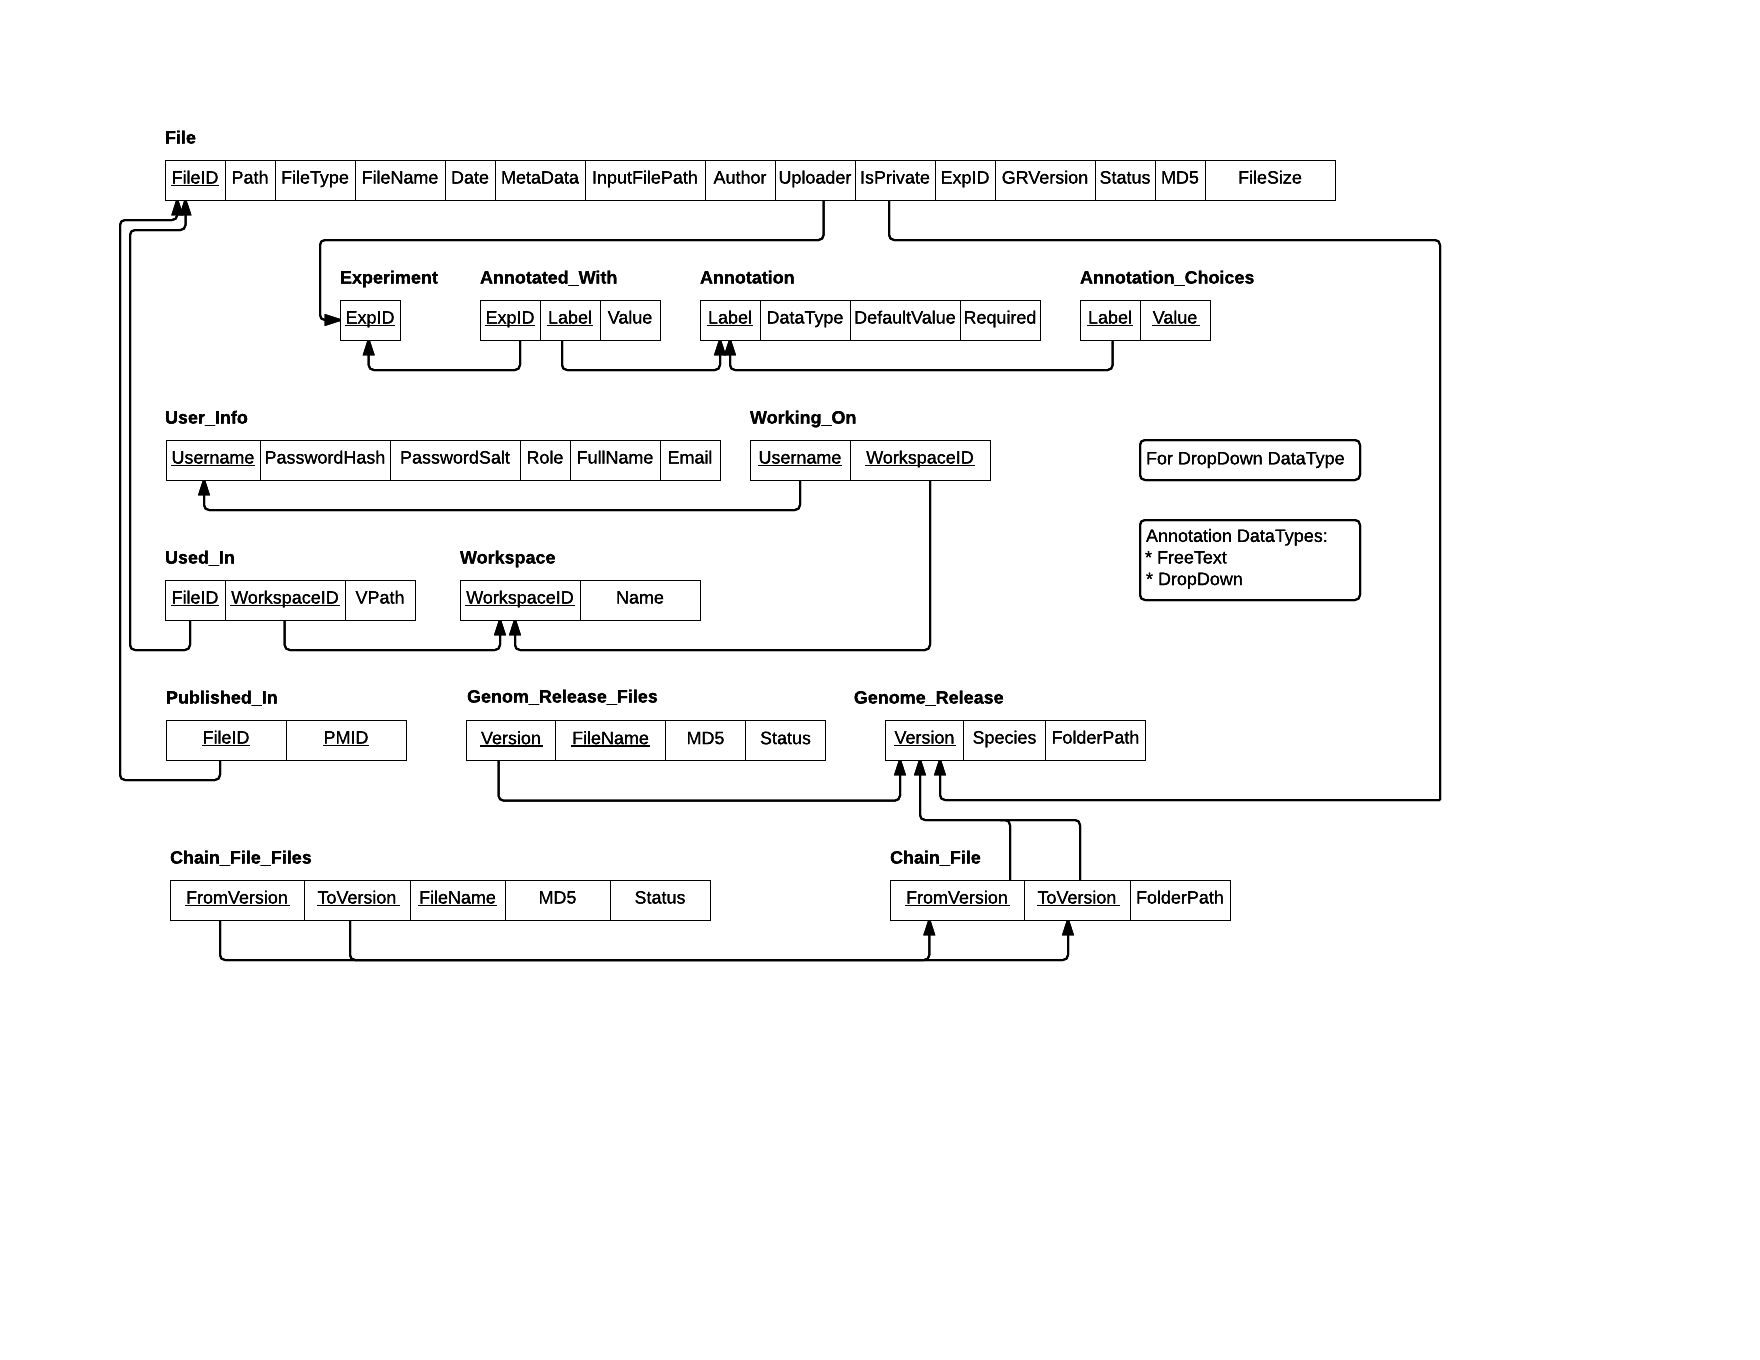
\includegraphics[width=20cm, angle=90, keepaspectratio=true]{dat_database_schema_v3.png}
%\addImageVertical{dat_database_schema_v3.png}
\caption{The database schema}
\label{fig:dat_databaseSchema}
\end{figure}

\FloatBarrier

\subsection{Database Design}
The following section will explain the less obvious columns and their intended use.

\texttt{FileID} is the identification number for a specific file. The data type \texttt{SERIAL} is used and will therefore be auto--generate unique identifiers upon insertion.

\texttt{Path} is the path to the corresponding file in the file system, for example: \\
\texttt{/var/www/data/Experiment1/raw/rawFile1.fastq}

\texttt{MetaData} is the string of parameters used in processing and should be \texttt{NULL} for all raw files.

\texttt{Annotated\_With} is the table that enables the annotation of experiments. The annotation in this table references the \texttt{Annotation}-table, to verify that new annotations are valid.

\begin{example}
To set the Species-annotation to ''Dog'' for the experiment Experiment1, the following tuple would be inserted into the Annotated\_With--table:
  \begin{center}
    \begin{tabular}{| l | l | l |}
      \hline
        \cellcolor{blue!25} ExpID & \cellcolor{blue!25} Label & \cellcolor{blue!25} Value \\
      \hline
      Experiment1 & Species & Dog \\
      \hline
      
    \end{tabular}
  \end{center}
\end{example}

\texttt{Annotation} is the table containing all the possible annotations a user can use to provide extra information about an experiment. This includes the type of annotation which is \term{Drop Down} for annotations where the user can choose from a drop down list, or \term{Free Text} where the user can enter the value freely. There is also support for a default value and annotation forcing where users are forced to provide the information. For \term{Drop Down} annotations the table \texttt{Annotation\_choices} specifies the valid choices.

The \texttt{Genome\_Release} table stores information about the \term{Genome Releases} available for use. This includes the unique version code for a \term{Genome Release}\cite{UCSCGRVERSION}. The \texttt{Genome\_Release\_Files} table stores the information about the files that make up the \term{Genome Release}.

\subsection{The Data Storage Subsystem}
All the classes used in the manipulation of the database and the creation of the file systems directory structure is contained in the java project's \texttt{database} package.

The other \appName\ subsystems execute all updates to the data storage through the \class{DatabaseAccessor} class. As a result there are many methods in this class, however most methods forwards the request to one of the classes in the \texttt{database.subclasses} package. Here the methods that modify the different areas of the data storage system are separated into different classes of more manageable sizes. An UML diagram of the \class{DatabaseAccessor} class and its subclasses is available in \refer{fig:dat_dbac} in  \refer{chap:dat_umls}.

The \class{DatabaseAccessor} utilizes a number of classes in order to return information to the method caller. These classes are contained in the \texttt{database.containers} package and are as follows:
\begin{itemize}
\item \class{Experiment}
\item \class{FileTuple}
\item \class{Annotation}
\item \class{Genome}
\end{itemize}

An UML diagram of these classes is also available in \refer{fig:dat_containers} in \refer{chap:dat_umls}.

\subsection{Interaction}
Below are examples of typical interactions with the \class{DatabaseAccessor} class.

\subsubsection{Adding an experiment}
In order to add an annotated experiment the following steps must be followed:
\begin{enumerate}
\item First the \term{addExperiment} method must be called. This will add one experiment to the database without any annotations set for that experiment. If you try to add one experiment that already exist then the addition will be refused and an exception will be thrown.

\item If there are no annotations that can be used to provide extra information about the experiment they must first be added by calling the \term{addFreeTextAnnotation} or \term{addDropDownAnnotation} methods.

\subitem If a \term{Drop Down} annotation already exists, but there is no suitable choice for the experiment a choice can be added by calling the \term{addDropDownAnnotationValue} method.

\item An available annotation can be used to provide extra information about an experiment by calling the \term{annotateExperiment} method.
\end{enumerate}

Now that an experiment has been added files can be added added to it.

\subsubsection{Annotation Handling}

Annotations can be handled using the methods below.

\begin{tabular}{|l| p{7cm}|}
\hline
\term{getChoices} & gets all the available annotation choices connected to a specific label. For example the possible choices returned for the label "sex" might be "Male, Female and Unknown". \\ \hline

\term{getAnnotations} & returns all annotation labels currently stored in the database. Examples could be "Sex,Species,Tissue,etc.". \\ \hline

\term{getAllAnnotationObjects} & Combines the two previous methods. Here an annotation object is returned that holds all the relevant information including the label, datatype, and the possible choices for a \term{Drop Down} annotation. \\ \hline

\term{changeAnnotationLabel} & updates the given label in the database. This will change the label for all experiments that use it. For example changing "specie" to "Species". \\ \hline

\term{changeAnnotationValue} & updates a value for a specific annotation label. For example changing "Human" to "Homosapien".  \\ \hline

\term{updateExperiment} & Updates an annotation for one specific experiment. Example: "experiment1, Species, Homosapien" can be changed to "experiment1, Species, Fly". \\ \hline

\term{deleteAnnotation} & deletes an unused annotation from the database. This will also delete all the choices for that annotation. \\ \hline

\term{removeAnnotationValue} & removes a single annotation value for a particular label. \\ \hline

\end{tabular}

\subsubsection{File Handling}
The actions of adding and deleting experiment files or genome releases can be performed using the following methods.

\begin{tabular}{|l| p{7cm}|}
\hline
\term{addNewFile} & To add a file you will need to have an experiment added before you call the \term{addNewFile} method. Raw files usually come in pairs and so they can be added together by specifying the input file name. \\ \hline

\term{deleteFile} & Deletes the given file from both the database and the file system. This can be done by either specifying the path or the file's ID number. \\ \hline

\term{addGenomeRelease} & Genome release files must be added one at a time by calling the \term{addGenomeRelease} method. This method returns an upload URL. \\ \hline

\term{removeGenomeRelease} & \term{removeGenomeRelease} removes all the files associated with a genome release. This can only be done if there are no files that have been generated using the specified genome release. \\ \hline
\end{tabular}
The Apache HTTP Server, or commonly referred to as Apache, is the web server application which is used to upload and download files to and from the server. Apache is open source, which makes it free to use. Apache is a good choice because it is developed and maintained by an open community, that way all new versions and updates will become available for free. Since it is open source, the source code is open for everyone to read. Apache can be used on both Unix/Windows systems. In this case it is running on a Unix machine but can still communicate with all platforms. 


%Write about proxy usage and such


\end{document}